\documentclass[a4paper,10pt,oneside,final,titlepage,onecolumn]{article}

\usepackage{ucs}
\usepackage[portuguese]{babel}
\usepackage[utf8x]{inputenc}
\usepackage[T1]{fontenc}
\usepackage{textcomp}
\usepackage{graphicx}
\usepackage{placeins}

\usepackage{listings}
\usepackage{color}

\definecolor{dkgreen}{rgb}{0,0.6,0}
\definecolor{gray}{rgb}{0.5,0.5,0.5}
\definecolor{mauve}{rgb}{0.58,0,0.82}

\lstset{frame=tb,
  language=bash,
  aboveskip=3mm,
  belowskip=3mm,
  showstringspaces=false,
  columns=flexible,
  basicstyle={\scriptsize\ttfamily},
  numbers=none,  
  breaklines=true,
  breakatwhitespace=true
  tabsize=3
}



\title{Exercício 5 de MC833 --- Programação em Redes de Computadores}
\author{Raul Rabelo Carvalho, 105607, turma A}



\begin{document}



\maketitle



\section{}
\paragraph{}O servidor pôde responder com um eco dos treze clientes como mostrado na figura \ref{echo}, pois, na verdade, ele o faz em sequência. A função \verb|select|\footnote{Stevens, W. Richard. Unix Network Programming, volume 1. Second Edition, pp. 150-155.} empregada no servidor marca em um vetor de bits (do tipo \verb|fd_set|) as conexões que o \emph{kernel} recebeu (já que, no caso do servidor deste exercício, faz-se somente leituras). As funções \verb|read| e \verb|write| usam a posição no vetor como descritor, já que este inteiro equivale aos descritores que o \emph{kernel} criou. Assim, fazendo uma iteração rápida sobre as posições do vetor marcadas com conexões ativas, o servidor, para efeitos práticos, trata as requisições dos clientes simultaneamente.
\begin{figure}[!ht]
  \caption{Servidor respondendo a treze clientes.}
  \centering
  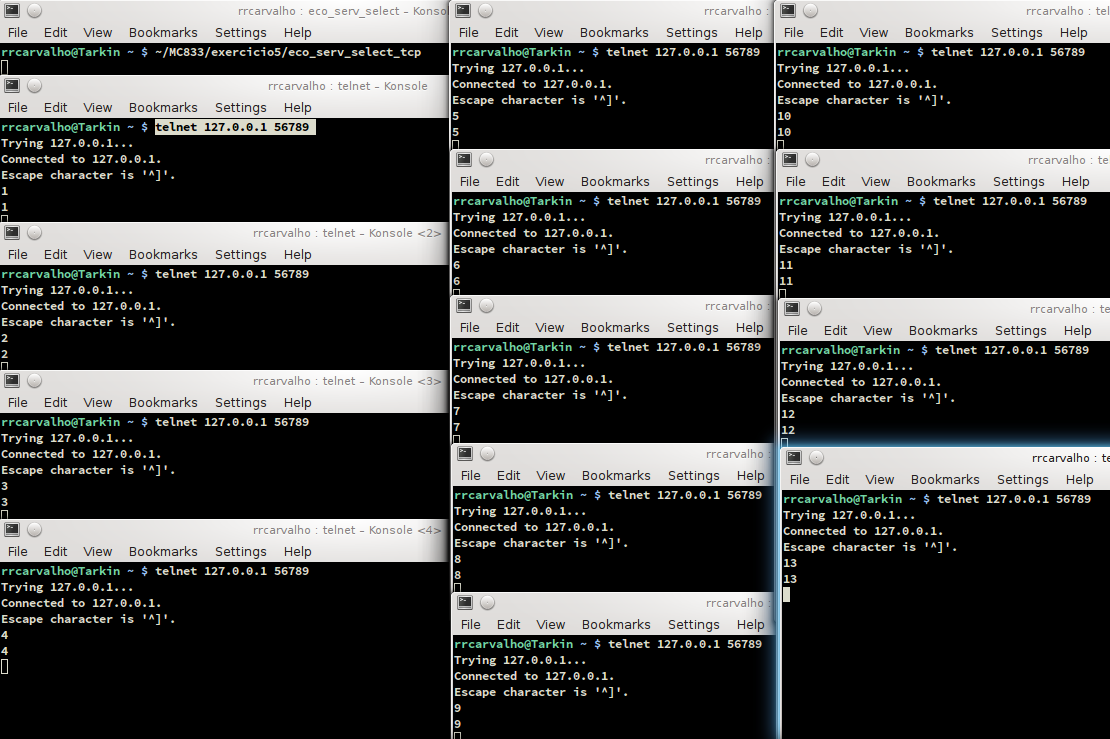
\includegraphics[width=150mm]{images/echo.png}
  \label{echo}
\end{figure}



\FloatBarrier
\section{}
\paragraph{}Como visto no exercício 4 desta disciplina, um servidor concorrente pode empregar a chamada de sistema \verb|fork| dos sistemas Unix para criar uma cópia própria para tratar de conexões simultâneas. Já um servidor por multiplexação de entrada e/ou saída não faz cópias de si próprio, mas emprega a capacidade de um \emph{kernel} Unix em gerenciar diversos descritores de entrada e saída por processo.
\paragraph{}O \emph{kernel} Unix pode gerenciar virtualmente um número ilimitado de descritores de E/S, dependente somente da memória alocada para cada descritor. No entanto, existe um limite \emph{hardwired} de 1024, que é o valor da macro \verb|FD_SETSIZE|\footnote{Stevens, W. Richard. Unix Network Programming, volume 1. Second edition, pp. 154-155.}. Este valor pode ser alterado, mas para que o sistema utilize do novo valor, o \emph{kernel} precisa ser recompilado. Há outro problema no fato da iteração sobre o total de descritores: se este valor aumentar muito, a interação pode se tornar demorada e o tempo de resposta de cada conexão pode aumentar, mitigando a impressão de simultaneidade das conexões.
\paragraph{}No entanto, a solução com o \verb|fork| pode sofrer perdas de desempenho ainda maiores, pois o efeito de simultaneidade também é conseguido por um tipo de iteração, neste caso o escalonamento de processos pelo sistema. Quando o número de processos filhos do servidor, cada um atentendo a uma conexão aumenta muito, o atraso devido a troca de contexto pode se tornar um fator que piora o desempenho. Outro problema é que cada processo filho tem uma cópia de todo contexto de execução do servidor, ocupando mais memória no \emph{host} que o servidor multiplexado com a pilha e o \emph{heap} de cada processo.
\paragraph{}Deste modo, a solução para múltiplas conexões ao servidor por multiplexação tem uma melhor capacidade de escalabilidade, pelo menos até o limite de 1024 conexões por servidor, já que incorre de um gasto menor de memória e ciclos (troca de contexto) da máquina hospedeira.



\end{document}
